\documentclass[12pt]{rowanthesis}
% \usepackage{packagename} % Add additional packages like this
\usepackage{algorithm}
\usepackage{algpseudocode}

% Preamble (PLEASE FILL IN ALL OF THE INFORMATION)
%------------------------------------------------------------------------%
\title{A NEW ALGORITHM FOR ENCOUNTER GENERATION: ENCOUNTERS FROM ACTUAL TRAJECTORIES (EnAcT)}
\author{James A. Ritchie III} 
\doclevel{Thesis}
\department{Electrical and Computer Engineering}
\school{College of Engineering}
\degree{Master of Science in Electrical and Computer Engineering}
\dateofdefense{October 31, 2023}
\chair{Nidhal Bouaynaya, Ph.D., Associate Dean for Research and Graduate Studies and Professor, Department of Electrical and Computer Engineering}
\chairsimple{Example Professor Name, Ph.D.}
\committeememberone{Ravi Ramachandran, Ph.D., Professor, Department of Electrical and Computer Engineering}
\committeemembertwo{Mike Paglione, Manager, Aviation Research Division, Office of Next Gen, Federal Aviation Administration }
\copyrightyear{2023}
\academicyear{2023-2024}
%------------------------------------------------------------------------------%

% Document body
%------------------------------------------------------------------------%
\begin{document}

% Title Page and Copyright Page
\makeTitlePage

% Dedications Page

\begin{center}
\textbf{Dedications}
\end{center}

I would like to dedicate this thesis to my wife, Tiffany Ritchie, our baby on the way, and my stepson Maddox Pino. My family has pushed me to finish my master’s and allow me to follow my dreams and complete my education. They have been there for me through everything, and I appreciate and love them so much.

\newpage 

% ---Front of report (pages numbered in Roman Numerals)---%
\begin{frontmatter}
    % Acknowledgements(s) Page (Optional)
    
\begin{center}
\textbf{Acknowledgements}
\end{center}

First and foremost, I would like to thank Deepak Chauhan and the branch he works for, FAA NextGen Surveillance Branch (ANG-C33) for funding the research for this thesis with the FAA Cooperative Agreement No. 15-G-001, which was awarded to Rowan University.

I would also like to thank Andrew Fabian of the FAA NextGen Unmanned Aircraft Systems Branch, ANG-C35 (formerly the Modeling and Simulation Branch, ANG-C55), for his expertise and insight into flight mechanics, bearing calculations, and overall algorithm derivation expertise. This work would not have been able to be completed without you, and I sincerely thank you for that and being a good friend and coworker.

I am very fortunate and grateful to Mike Paglione, who guided this project and research from the FAA standpoint. You are a great manager, and I am thankful that I had the privilege to work under you, and to learn so much from you and others in the branch.

To Dr. Bouaynaya, thank you for your patience in completing this thesis, and for the expertise and knowledge in support of this work. I learned so much from your teachings, and I cannot thank you enough for everything. 

Not least of all, I owe thanks to my wife, stepson, mentors, and friends for their support and patience as I completed this thesis. I cannot name everyone, as it would take a lifetime to write, and too many pages to fill, but I want you all to know how thankful I am. Thank you everyone.


\newpage
    
    % Abstract
    \buildAbstract
    
    % TOC, LOF and LOT
    \buildTOC
    \buildListOfFigures
    \buildListOfTables
\end{frontmatter}
%----------------------------------------------------------%

% ---Body of report (pages numbered in Arabic Numerals)---%
\begin{thesisbody}
    
\chapter{Introduction}

The Federal Aviation Administration (FAA) and private industry collectively within the Radio Technical Commission for Aeronautics (RTCA) Special Committee (SC) 228 are working to define the minimum operational performance standards (MOPS) for unmanned aircraft systems (UAS) to allow for safe integration of UAS into the National Airspace System (NAS). Part of defining the MOPS is ensuring the Detect and Avoid Algorithms (DAA) on UAS function properly to adhere to the See and Avoid requirement of the 14 CFR 91 - General Operating and Flight Rules imposed by the FAA. The FAA Federal Aviation Regulation (FAR) requirement of “See and Avoid” is essential to safe flight in manned aircraft. See and Avoid refers to the ability of the pilot to visually scan the surrounding airspace and determine possible risks. It is then the pilot's responsibility to avoid these risks by following the rules defined in the FAR or by any means in the case of an emergency. Thus, UASs without a pilot on board the aircraft are required to carry DAA systems that comply with 14 CFR 91.

The DAA system provides preventive, corrective, and warning guidance to the UAS pilot to assist in preventing loss of separation with other aircraft. These systems have significant technical challenges in establishing and maintaining the relative position of one or more external threats (i.e., aircraft) during an encounter. The entire DAA system consists of surveillance sensors used to detect an intruder, tracker to fuse and filter multiple sources of information to provide one single track to the DAA algorithm.

To ensure DAA systems can detect other aircraft, the systems need to be tested. Evaluating these systems requires scenarios in which two or more aircraft have a close encounter with each other. An encounter event is when two aircraft of interest are within a defined range of each other, typically close enough to cause a concern with air traffic control. A subset of encounters, called conflicts, are legally defined as a loss of separation between the two aircraft. Encounter/Conflict definitions change with the different types of airspaces in the NAS. In EnRoute (Class A) airspace, separation distances are usually greater than those in terminal (Class B, C, D, E) airspaces. The DAA system must be tested with cases of encounters and conflicts in all airspace types to ensure they can correctly identify when the UAS may stray too close to another aircraft. This work focuses on encounters with two aircraft.

In the NAS, no conflicts exist since the controllers keep the traffic separated thus preventing the use of unmodified recorded air traffic. Scenarios need to be generated to be able to simulate these desired encounters. Current capabilities of generating rely on simulated input traffic scenarios based on either simple linear aircraft trajectories or recorded traffic scenarios \cite{oaks:2001, paglione:2003, oaks:2002a, oaks:2002b, ritchie:2016}. However, these approaches are either limited by the simplicity of their models or by the breadth of the traffic recordings available. Thus, there is a need for more realistic and complex algorithms to generate a large set of user specified traffic scenarios.

In the literature, the generation of conflicting aircraft trajectories can be divided into three categories: (1) fitting probabilistic distributions and statistical models over the range of encounter variables \cite{kochenderfer-correlated:2008, kochenderfer-uncorrelated:2008}; (2) using recorded air-traffic data through time-shifting the flights \cite{oaks:2001, paglione:2003, oaks:2002a, oaks:2002b, ritchie:2016}; and (3) ad-hoc generation of aircraft trajectories for the main purpose of studying conflict detection \cite{malaek:2011, ming:2011, meng:2012, liu:2014, yang:2017}. Each of these approaches considers different assumptions and addresses different concerns regarding what type of conflicts are generated and why they are needed.

The encounter model in \cite{kochenderfer-correlated:2008}, developed by the Massachusetts Institute of Technology's (MIT) Lincoln Laboratory, describes a probabilistic aircraft encounter model. This model is currently limited to generating encounters in the EnRoute environment, where flights are typically cruising and do not change altitude often. Also, the encounters are all generated at random (according to the probabilistic properties), and you cannot specify what kind of encounter you would like to have. MIT Lincoln Laboratory is currently working on a new encounter model, but it is not ready for generating encounters at the time of this publication.

The FAA has traditionally generated aircraft conflicts and encounters through the use of time-shifting the flights in a recorded air traffic scenario \cite{oaks:2001, paglione:2003}. These algorithms consider the recorded flight data of aircraft that have flown in the NAS and shift the position of the aircraft in time to induce encounters. The resulting trajectories contain the same physical flight position data as the original recorded traffic data, but the aircraft fly these tracks at new times. A genetic algorithm was implemented to determine the optimal time-shift values for each flight in the scenario \cite{oaks:2002a}. Even though more encounter criteria have been considered \cite{oaks:2002b} and the algorithm has been improved since its original version \cite{ritchie:2016}, current algorithms only generate encounters from flights that have existed in the NAS. This prevents the user from specifying the exact parameters for each conflict, which is useful for testing specific conditions. These algorithms have only been tested on EnRoute (Class A) airspace, and not on data from the terminal environment. These methods would need to be evaluated for use in terminal environments and have had limited use beyond EnRoute airspace.

Other studies did not focus on the problem of aircraft conflict generation, but considered the issue of conflict detection or resolution \cite{malaek:2011, ming:2011, liu:2014, yang:2017}. Aircraft conflicts in these studies are typically fixed and have only examined a subset of conflict types. The trajectories of these aircraft are typically straight, and use coordinates based on a flat-Earth system. While the encounter properties are typically specified, the method in which they are created is not conducive to generating millions of encounters in a reasonable time span. This paper addresses the need to simulate encounter traffic events for the aim of testing the DAA capabilities of UAS in all airspace types. 

In this paper, we propose an algorithm to calculate the bearing between two aircraft given a defined encounter scenario. Specifically, we propose a new algorithm that uses a spherical Earth model to retain accuracy in the calculation of the bearing between the aircraft in a defined encounter scenario. A program called Encounters from Actual Trajectories (EnAcT) was written to use this algorithm to generate encounters using the derived algorithm and the defined encounter properties. The output of the program will cover gaps that exist in the types of encounters that are needed for testing, including the use of performance parameters from EuroControl's Base of Aircraft Data (BADA) \cite{bada:v3} to generate pairs of 4D trajectories that satisfy a specified set of encounter event properties. 

To determine the encounter properties that would be realistic to what is found in the NAS, a study was performed during this work to determine these values. Statistical distributions were created from real-world data for each encounter property and used by the program that was developed to generate numerous encounters that would be realistic. This allows the FAA to test UAS DAAs based on what is more likely to be found in actual air traffic operations.

    \chapter{Mathematical Formulation and Algorithm}
\label{chap:math}

We define an encounter between two aircraft: an ownship and an intruder. Ownship has an arbitrarily defined latitude, longitude, altitude, and heading:
\begin{equation}
    \phi_{O,CPA} \ \ \lambda_{O,CPA} \ \ h_{O,CPA} \ \ \theta_{O,CPA}
\end{equation}
The intruder will be located at:
\begin{equation}
    \begin{aligned}
        \phi_{I,CPA} \ \ \lambda_{I,CPA} \ \ &h_{O,CPA} \mp D_{V,CPA} \ \ \theta_{O,CPA} \\
        &+ \Delta \theta_{CPA} \ \ dist(\phi_{O,CPA} \ \ \lambda_{O,CPA} \ \ \phi_{I,CPA} \ \ \lambda_{I,CPA}) \\
        &= D_{H,CPA}
    \end{aligned}
\end{equation}
We can express latitude and longitude as a unit normal vector:
\begin{equation}
    N = (\cos{\phi}\cos{\lambda} \ \ \ \cos{\phi}\sin{\lambda} \ \ \ \sin{\phi})
\end{equation}
Let \(\pi_{i}(N)\) be the projection function that selects the \(i^{th}\) component of vector \(N\). We can find the north \(\hat{v}\) and east \(\hat{\epsilon}\) unit vectors at \(N\) to be:
\begin{equation}
    \begin{aligned}
        \hat{v} &= \frac{(-\pi_{1}(N)\pi_{3}(N) \ \ \ -\pi_{2}(N)\pi_{3}(N) \ \ \ \pi_{1}{}^{2}(N) + \pi_{2}{}^{2}(N))}{\sqrt{\pi_{1}{}^{2}(N)+\pi_{2}{}^{2}(N)}} \\
        &= (-\sin{\phi}\cos{\lambda} \ \ \ -\sin{\phi}\sin{\lambda} \ \ \ \cos{\phi})
    \end{aligned}
\end{equation}
\begin{equation}
    \hat{\epsilon} = \frac{(-\pi_{2}(N) \ \ \ \pi_{1}(N) \ \ \ 0)}{\sqrt{\pi_{1}{}^{2}(N)+\pi_{2}{}^{2}(N)}} = (-\sin{\lambda} \ \ \ \cos{\lambda} \ \ \ 0)
\end{equation}
For any heading \(\theta\) and central angle \(c\), we know the formula to give us the endpoint’s unit normal vector:
\begin{equation}
    N_{end} = N_{start}\cos{c} + (\hat{v}\cos{\theta} + \hat{\epsilon}\sin{\theta})\sin{c}
\end{equation}
Let \(\hat{D} = (\hat{v}\cos{\theta}+\hat{\epsilon}\sin{\theta})\) be the directional unit vector. We also know how to interpolate points on a great circle in two ways:
\begin{equation}
    N(t) = N_{start}\frac{\sin{(c-c(t))}}{\sin(c)} + N_{end}\frac{\sin{c(t)}}{\sin{c}}
\end{equation}
or
\begin{equation}
    N(t) = N_{start}\cos{c(t)} + \frac{N_{end}-N_{start}\cos{c}}{\sin{c}}\sin{c(t)}
\end{equation}
We can see that it is easy to move between these two formulae:
\begin{equation}
    \frac{N_{end}-N_{start}\cos{c}}{\sin{c}} = (\hat{v}\cos{\theta + \hat{\epsilon}}\sin{\theta}) = \hat{D}
\end{equation}
If we have a fixed start point and a fixed arc-distance to travel \(r\), we have an equation for all points equidistant from a reference point (a circle of radius \(r\)):
\begin{equation}
    N_{circle}(x) = N_{center}\cos{r} + (\hat{v}\cos{x} + \hat{\epsilon}\sin{x})\sin{r}
\end{equation}
Let \(\hat{B}(x) = (\hat{v}\cos{x} + \hat{\epsilon}\sin{x})\) be the bearing vector for bearing \(x\). At CPA, we can express the horizontal position of the intruder in terms of a circle around the ownship:
\begin{equation}
\label{eq:nicpa}
    N_{I,CPA}(x) = N_{O,CPA}\cos{\frac{D_{H,CPA}}{R}} + \hat{B}_{CPA}(x)\sin{\frac{D_{H,CPA}}{R}}
\end{equation}
We know the parameterization of both tracks horizontally:
\begin{equation}
    N_{O}(t) = N_{O,CPA}\cos{\left( \frac{v_{T,O}}{R}(t-t_{CPA}) \right)} + \hat{D}_{O,CPA}\sin{\left( \frac{v_{T,O}}{R}(t-t_{CPA}) \right)}
\end{equation}
\begin{equation}
    N^{'}_{O}(t) = \frac{v_{T,O}}{R} \left(-N_{O,CPA} \sin{\left( \frac{v_{T,O}}{R}(t-t_{CPA}) \right)} + \hat{D}_{O,CPA}\cos{\left( \frac{v_{T,O}}{R}(t-t_{CPA}) \right)} \right)
\end{equation}
\begin{equation}
    N_{I}(x,t) = N_{I,CPA}\cos{\left( \frac{v_{T,I}}{R}(t-t_{CPA}) \right)} + \hat{D}_{I,CPA}\sin{\left( \frac{v_{T,I}}{R}(t-t_{CPA}) \right)}
\end{equation}
\begin{equation}
    \frac{\partial N_{I}(x,t)}{\partial t} = \frac{v_{T,I}}{R} \left(-N_{I,CPA} \sin{\left( \frac{v_{T,I}}{R}(t-t_{CPA}) \right)} + \hat{D}_{I,CPA}\cos{\left( \frac{v_{T,I}}{R}(t-t_{CPA}) \right)} \right)
\end{equation}
At CPA, these are:
\begin{equation}
    N_{O}(t_{CPA}) = N_{O,CPA}
\end{equation}
\begin{equation}
    N^{'}(t_{CPA}) = \frac{v_{T,O}}{R}\hat{D}_{O,CPA}
\end{equation}
\begin{equation}
    N_{I}(x,t_{CPA}) = N_{I,CPA}(x) 
\end{equation}
\begin{equation}
    \left. \frac{\partial N_{I}(x,t)}{\partial t} \right|_{t=t_{CPA}} = \frac{v_{T,I}}{R}\hat{D}_{I,CPA}
\end{equation}
Now remember horizontal distance is measured as:
\begin{equation}
    H(x,t) = 2R\arcsin{\frac{||N_{I}(x,t)-N_{O}(t)||}{2}}
\end{equation}
and its derivative is:
\begin{equation}
    \frac{\partial H(x,t)}{\partial t} = \frac{R(||N_{I}(x,t)-N_{O}(t)||)^{'}}{\sqrt{1-\left( \frac{||N_{I}(x,t)-N_{O}(t)||}{2} \right)^{2}}}
\end{equation}
where:
\begin{equation}
    (||N_{I}(x,t)-N_{O}(t)||)^{'} = \frac{(N_{I}-N_{O}) \cdot \frac{\partial (N_{I}-N_{O})}{\partial t}}{||N_{I}-N_{O}||} = \frac{(N_{I}-N_{O}) \cdot \left( \frac{\partial N_{I}}{\partial t} - N^{'}_{O}\right)}{||N_{I}-N_{O}||}
\end{equation}
We know:
\begin{equation}
    N_{I} \cdot \frac{\partial N_{I}}{\partial t} = \frac{v_{T,I}}{R}\cos{\left( 2\frac{v_{T,I}}{R}(t-t_{CPA} \right)}(N_{I,CPA} \cdot \hat{D}_{I,CPA}) = 0
\end{equation}
Therefore:
\begin{equation}
    \begin{aligned}
        (N_{I}-N_{O}) \cdot \left( \frac{\partial N_{I}}{\partial t} - N^{'}_{O} \right) &= N_{I} \cdot \frac{\partial N_{I}}{\partial t} - N_{I} \cdot N^{'}_{O} - N_{O} \cdot \frac{\partial N_{I}}{\partial t} + N_{O} \cdot N^{'}_{O} \\
        &= - \left( N_{I} \cdot N^{'}_{O} + N_{O} \cdot \frac{\partial N_{I}}{\partial t} \right)
    \end{aligned}
\end{equation}
So:
\begin{equation}
    \frac{\partial H(x,t)}{\partial t} = -R\frac{N_{I}(x,t) \cdot N^{'}_{O}(t) + N_{O}(t) \cdot \frac{\partial N_{I}(x,t)}{\partial t}}{|| N_{I}(x,t) - N_{O}(t) || \sqrt{1 - \left( \frac{|| N_{I}(x,t) - N_{O}(t) ||}{2} \right)^{2}}}
\end{equation}
We also know the chord length is directly related to the central angle as:
\begin{equation}
    H(x,t) = 2R\arcsin{\frac{|| N_{I}(x,t) - N_{O}(t) ||}{2}}
\end{equation}
Therefore:
\begin{equation}
    ||N_{I}(x,t) - N_{O}(t)|| = 2\sin{\frac{H(x,t)}{2R}}
\end{equation}
By substituting into the denominator:
\begin{equation}
    \begin{aligned}
        ||N_{I}(x,t)-N_{O}(t)||& \sqrt{1- \left( \frac{||N_{I}(x,t)-N_{O}(t)||}{2} \right)^{2}} \\
        &= 2\sin{\frac{H(x,t)}{2R}}\sqrt{1-sin{^{2}\frac{H(x,t)}{2R}}} \\
        &= \sin{\frac{H(x,t)}{R}}
    \end{aligned}
\end{equation}
\begin{equation}
    \frac{\partial H(x,t)}{\partial t} = -R \frac{N_{I}(x,t) \cdot N^{'}_{O}(t) + N_{O}(t) \cdot \frac{\partial N_{I}(x,t)}{\partial t}}{\sin{\frac{D_{H,CPA}}{R}}}
\end{equation}
At CPA, this becomes:
\begin{equation}
    -\frac{v_{T,I}N_{O,CPA} \cdot \hat{D}_{I,CPA}(x) + v_{T,O}N_{I,CPA}(x) \cdot \hat{D}_{O,CPA}}{\sin{\frac{D_{H,CPA}}{R}}}
\end{equation}
However,
\begin{equation}
    \frac{N_{I,CPA}(x)}{\sin{\frac{D_{H,CPA}}{R}}} = N_{O,CPA}\cot{\frac{D_{H,CPA}}{R}} + \hat{B}_{CPA}(x)
\end{equation}
And
\begin{equation}
    \begin{aligned}
        &\left( N_{O,CPA}\cot{\frac{D_{H,CPA}}{R}} + \hat{B}_{CPA}(x) \right) \cdot \hat{D}_{O,CPA} \\
        &= \cot{\frac{D_{H,CPA}}{R}} N_{O,CPA} \cdot \hat{D}_{O,CPA} + \hat{B}_{CPA}(x) \cdot \hat{D}_{O,CPA}
    \end{aligned}
\end{equation}
But remember \( N_{O,CPA} \cdot \hat{D}_{O,CPA} = 0 \) so:
\begin{equation}
    \begin{aligned}
        \frac{N_{I,CPA}(x)}{\sin{\frac{D_{H,CPA}}{R}}} = &\hat{B}_{CPA}(x) \cdot \hat{D}_{O,CPA} \\
        &= (\hat{v}_{O,CPA}\cos{x} + \hat{\epsilon}\sin{x}) \cdot (\hat{v}_{),CPA}\cos{\theta_{O,CPA}} + \hat{\epsilon}_{O,CPA}\sin{\theta_{O,CPA}}) \\
        &= \cos{x}\cos{\theta_{O,CPA}} + \sin{x}\sin{\theta_{O,CPA}} \\
        &= \cos{(x-\theta_{O,CPA})}
    \end{aligned}
\end{equation}
to get:
\begin{equation}
    - \left( \frac{v_{T,I}N_{O,CPA} \cdot \hat{D}_{I,CPA}(x)}{\sin{\frac{D_{H,CPA}}{R}}} + v_{T,O} \cos{(x-\theta_{O,CPA})} \right)
\end{equation}
Now we can calculate \(N_O,CPA \cdot \hat{v}_I,CPA\):
\begin{equation}
    \begin{aligned}
        &N_{O,CPA} \cdot \hat{v}_{I,CPA} \\
        &= N_{O,CPA} \\ \cdot
        & \frac{(-\pi_{1}(N_{I,CPA})\pi_{3}(N_{I,CPA}) \ \ \ -\pi_{2}(N_{I,CPA})\pi_{3}(N_{I,CPA}) \ \ \ \pi_{1}{}^{2}(N_{I,CPA}) + \pi_{2}{}^{2}(N_I,CPA))}{\sqrt{\pi_{1}{}^{2}(N_{I,CPA}) + \pi_{2}{}^{2}(N_{I,CPA})}}
    \end{aligned}
\end{equation}
Completing the dot-product produces the following in the numerator:
\begin{equation}
    \begin{aligned}
        -\pi_{1}(N_{O,CPA})&\pi_{1}(N_{I,CPA})\pi_{3}(N_{I,CPA}) - \pi_{2}(N_{O,CPA})\pi_{2}(N_{I,CPA})\pi_{3}(N_{I,CPA}) \\
        &+ \pi_{3}N_{O,CPA}(\pi_{1}{}^{2}(N_{I,CPA}) + \pi_{2}{}^{2}(N_{I,CPA})
    \end{aligned}
\end{equation}
Simplifying the numerator, we get:
\begin{equation}
    \begin{aligned}
        &\pi_{3}(N_{O,CPA}) - \pi_{3}(N_{I,CPA}) \cdot \\ 
        &(\pi_{1}(N_{O,CPA})\pi_{1}(N_{I,CPA}) + \pi_{2}(N_{O,CPA})\pi_{2}(N_{I,CPA}) + \pi_{3}(N_{O,CPA})\pi_{3}(N_{I,CPA}))
    \end{aligned}
\end{equation}
We can further simplify and get the whole equation as:
\begin{equation}
    = \frac{\pi_{3}(N_{O,CPA})-\pi_{3}(N_{I,CPA})N_{O,CPA} \cdot N_{I,CPA}}{\sqrt{\pi_{1}{}^{2}(N_{I,CPA}) + \pi_{2}{}^{2}(N_{I,CPA})}}
\end{equation}
Knowing what \(N_{I,CPA}\) is equal to from \ref{eq:nicpa}, we can simply further:
\begin{equation}
    = \frac{\pi_{3}(N_{O,CPA})-\pi_{3}(N_{I,CPA})\cos{\frac{D_{H,CPA}}{R}}}{\sqrt{\pi_{1}{}^{2}(N_{I,CPA}) + \pi_{2}{}^{2}(N_{I,CPA})}}
\end{equation}
We can substitute \(N_{I,CPA}\) with \ref{eq:nicpa} to reintroduce our unknown (\(x\)) back into the equation:
\begin{equation}
    = \frac{\pi_{3}(N_{O,CPA})\sin{\frac{D_{H,CPA}}{R}}-\pi_{3}(\hat{B}_{CPA}(x))\cos{\frac{D_{H,CPA}}{R}}}{\sqrt{\pi_{1}{}^{2}(N_{I,CPA}) + \pi_{2}{}^{2}(N_{I,CPA})}}\sin{\frac{D_{H,CPA}}{R}}
\end{equation}
We can replace the remaining \(N_{O,CPA}\) and \(N_{I,CPA}\) terms and the \(\hat{B}_{CPA}(x)\) term with their equivalents to only have one unknown (\(x\)):
\begin{equation}
    = \frac{\sin{\phi_{O,CPA}}\sin{\frac{D_{H,CPA}}{R}}-\cos{\phi_{O,CPA}}\cos{\frac{D_{H,CPA}}{R}}\cos{x}}{\sqrt{1- \left(\sin{\phi_{O,CPA}}\cos{\frac{D_{H,CPA}}{R}} + \cos{\phi_{O,CPA}}\sin{\frac{D_{H,CPA}}{R}}\cos{x} \right) }}\sin{\frac{D_{H,CPA}}{R}}
\end{equation}
Now, we can calculate east direction:
\begin{equation}
    N_{O,CPA} \cdot \hat{\epsilon}_{I,CPA} = N_{O,CPA} \cdot \frac{(-\pi_{2}(N_{I,CPA}) \ \ \ \pi_{1}(N_{I,CPA}) \ \ \ 0)}{\sqrt{\pi_{1}{}^{2}(N_{I,CPA}) + \pi_{2}{}^2(N_{I,CPA})}}
\end{equation}
Completing the dot-product, we get:
\begin{equation}
    = \frac{\pi_{2}(N_{O,CPA})\pi_{1}(N_{I,CPA})-\pi_{1}(N_{O,CPA})\pi_{2}(N_{I,CPA})}{\sqrt{\pi_{1}{}^{2}(N_{I,CPA})+\pi_{2}{}^{2}(N_{I,CPA})}}
\end{equation}
Utilizing \ref{eq:nicpa}, we can bring in our unknown (\(x\)):
\begin{equation}
    =\frac{\pi_{2}(N_{O,CPA})\pi_{1}(\hat{B}_{CPA}(x))-\pi_{1}(N_{O,CPA})\pi_{2}(\hat{B}_{CPA}(x))}{\sqrt{\pi_{1}{}^{2}(N_{I,CPA})+\pi_{2}{}^{2}(N_{I,CPA})}} \sin{\frac{D_{H,CPA}}{R}}
\end{equation}
Replacing the remaining \(N_{O,CPA}\) and \(N_{I,CPA}\) terms and the \(\hat{B}_{CPA}(x)\) term like we did in the north vector yields:
\begin{equation}
    \begin{aligned}
        = (\cos{\phi_{O,CPA}}&\sin{\lambda_{O,CPA}})(-\sin{\phi_{O,CPA}}\cos{\lambda_{O,CPA}}\cos{x}-\sin{\lambda_{O,CPA}}\sin{x}) \\
        &-(\cos{\phi_{O,CPA}}\cos{\lambda_{O,CPA}})(-\sin{\phi_O,CPA}\sin{\lambda_{O,CPA}}\cos{x} \\
        &+ \cos{\lambda_{O,CPA}}\sin{x})\sin{\frac{D_{H,CPA}}{R}} \\
        & / \sqrt{1 - \left( \sin{\phi_O,CPA}\cos{\frac{D_{H,CPA}}{R}} + \cos{\phi_{O,CPA}}\sin{\frac{D_{H,CPA}}{R}}\cos{x} \right)^{2}}
    \end{aligned}
\end{equation}
Simplifying we get:
\begin{equation}
    =-\frac{\cos{\phi_{O,CPA}}\sin{x}}{\sqrt{1-\left( \sin{\phi_{O,CPA}}\cos{\frac{D_{H,CPA}}{R}} + \cos{\phi_{O,CPA}}\sin{\frac{D_{H,CPA}}{R}}\cos{x} \right)^{2}}}\sin{\frac{D_{H,CPA}}{R}}
\end{equation}
Now we have:
\begin{equation}
    \begin{aligned}
        &\frac{N_{O,CPA} \cdot (\hat{v}_{I,CPA}\cos{\phi_{I,CPA}}+\hat{\epsilon}_{I,CPA}\sin{\theta_{I,CPA}})}{\sin{\frac{D_{H,CPA}}{R}}} \\
        &= \frac{\left( \sin{\phi_{O,CPA}}\sin{\frac{D_{H,CPA}}{R}} - cos{\phi_{O,CPA}}\cos{\frac{D_{H,CPA}}{R}}\cos{x} \right)\cos{\theta_{I,CPA}} - \cos{\phi_{O,CPA}}\sin{x}\sin{\theta_{I,CPA}}}{\sqrt{1-\left( \sin{\phi_{O,CPA}}\cos{\frac{D_{H,CPA}}{R}} + \cos{\phi_{O,CPA}}\sin{\frac{D_{H,CPA}}{R}}\cos{x} \right)^{2}}}
    \end{aligned}
\end{equation}
\begin{equation}
\label{eq:genform}
    \begin{aligned}
        &\left. \frac{\partial H(x,t)}{\partial t} \right|_{t=t_{CPA}} \\
        &= v_{T,I} \frac{a-b+c}{\sqrt{1-\left( \cos{\phi_{O,CPA}}\sin{\frac{D_{H,CPA}}{R}}\cos{x} + \sin{\phi_{O,CPA}}\cos{\frac{D_{H,CPA}}{R}} \right)^{2}}}\\
        &\quad - v_{T,O}\cos{(x-\theta_{O,CPA})}
    \end{aligned}
\end{equation}
where:
\begin{multline}
\label{eq:gennum}
    a = \cos{\phi_{O,CPA}}\cos{\frac{D_{H,CPA}}{R}}\cos{\theta_{I,CPA}}\cos{x} \\ 
    b = \sin{\phi_{O,CPA}}\sin{\frac{D_{H,CPA}}{R}}\cos{\theta_{I,CPA}} \\
    c = \cos{\phi_{O,CPA}}\sin{\theta_{I,CPA}}\sin{x}
\end{multline}
The final equation (\ref{eq:genform} with \ref{eq:gennum}) is an equation with one unknown, the bearing (\(x\)), which satisfies all CPA constraints. This will give you the starting locations for each aircraft in the general case. It guarantees that the aircraft are at the required distances, at a specified encounter angle and single set of speeds. The constraint can be numerically solved. The only consideration left is to determine if the solution is maximal or minimal. If it is maximal, I think either there is a solution near the opposite bearing, or the constraints of the system are most likely malformed, and a solution is not attainable. See \autoref{chap:verification} and \autoref{chap:x0} for a detailed example that proves the derived question.
    \chapter{EnAcT Program}
\label{chap:enactprogram}

The algorithm developed in \hyperref[chap:math]{Chapter 2 Mathematical Forumlation and Algorithm} is implemented in a Java program known as Encounters from Actual Trajectories (EnAcT). This program can be described with the pseudo-code given in \hyperref[alg:enactrun]{Algorithm 1}. Java was chosen as the language platform due to experience plus the ability to transfer the program to any computer capable of running Java.
~\\
~\\
\begin{algorithm}[H]
\caption{EnAcT Program Run Sequence}
\label{alg:enactrun}
\begin{algorithmic}

\State Read in inputs
\While{There exists defined encounters to generate or required number not met}
    \State Calculate bearing at CPA based on given inputs
    \If{Bearing exists}
        \State Determine heading of aircraft at CPA
        \State Build trajectories of each aircraft
        \State Print trajectories to file
    \Else
        \State Log that bearing could not be found
        \State Skip this set of inputs
    \EndIf
\EndWhile 
\end{algorithmic}
\end{algorithm}
~\\

This program accepts inputs in two formats: 1) each encounter is defined with each of its properties explicitly by the user; or 2) probability distributions for each encounter property is defined along with the number of encounters to generate. The probability distributions can be given so that all encounters generated will fit the given distributions. Either set of inputs can generate an unlimited number of encounter scenarios with synthetic trajectories that match the given performance model (BADA). The properties define the encounter at the closest point of approach (CPA), and are:
\begin{itemize}
    \item Horizontal Separation Distance at CPA
    \item Vertical Separation Distance at CPA
    \item Latitude of Ownship at CPA
    \item Longitude of Ownship at CPA
    \item Encounter Angle at CPA
    \item Aircraft types
    \item Vertical Phase of flight for both aircraft
    \item Number of encounters (if giving distributions)
\end{itemize}
The Java program uses \ref{eq:genform} and \ref{eq:gennum} to determine the bearing between two aircraft at the closest point of approach (CPA) based on the given inputs, which is step 3 in \hyperref[alg:enactrun]{Algorithm 1}. If a bearing can be found, the program then uses a trajectory engine, in this case BADA, to generate the trajectories of the two aircraft based on the initial starting point and the properties at CPA. The trajectories are then written out into a Comma Separated Value (CSV) file. If the bearing cannot be found, the attempt is skipped based on the given inputs, and is logged.
    \chapter{Process for Generating EnAcT Inputs}

EnAcT requires the distributions for each encounter property to be able to generate millions of encounters that fall into these distributions. To generate these distributions that are realistic to what can be seen in the NAS, the Modeling and Simulation Branch developed a process to determine these distributions. A software tool that the branch developed, called the Trajectory Conflict Probe \cite{paglione:2008}, is the first step of the process. It inputs recorded flight plans and surveillance position reports and predicts when two aircraft are on a path that could violate these separation distances. Air traffic controllers issue clearances to alter one or both aircraft’s paths to resolve these conflicts before they occur. The tool records both the initial event and when the conflict is resolved. This allows the team to determine theoretical encounters from recorded air traffic data that had no actual encounters occurring due to air traffic controller intervention. \ref{fig:tcp} shows the flow of the Trajectory Conflict Probe program. 

\begin{figure}
\centering
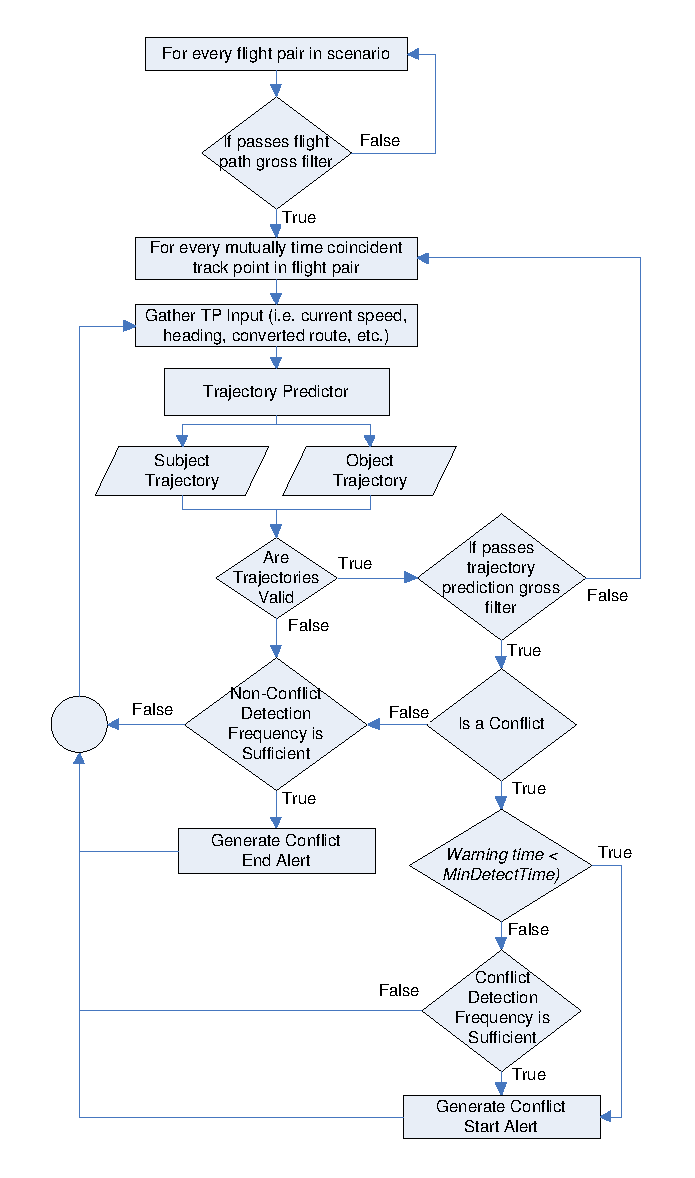
\includegraphics[scale=0.95]{Figures/TrajectoryConflictProbeFlowChart.pdf}
\caption{Flowchart of the Trajectory Conflict Probe Algorithm}
\floatfoot{\textit{Note.} This program analyzes each flight pair that has paths that are close enough to potentially cause a conflict \cite{paglione:2008}. Using a trajectory engine and the relevant clearance information, this program can predict where a conflict could have occurred if it were not for controller intervention, as long as the generated trajectories are valid.}
\label{fig:tcp}
\end{figure}

As \ref{fig:tcp} illustrates, the Trajectory Conflict Probe performs a pairwise analysis of flights from a given air traffic scenario. It considers each aircraft's flight plans, amendments, issued controller clearances, and surveillance position reports. The software first runs a gross filter to check rapidly for approximate temporal and spatial overlap of the pair of aircraft, based on the given position reports, or track data, of the two aircraft. This filter removes flight pairs that have no potential spatial overlap, cutting down the processing needed. If the pair passes this initial gross filter, the tool is called the Trajectory Predictor, which generates a predicted trajectory at each incremental time step that both aircraft have available track data. These predicted trajectories pass through a sequence of filters to determine if any predicted conflicts (violations of separation standards) or encounters (larger separation events) occur. 

Once an encounter is detected, the algorithm checks to see if the encounter occurs within the user defined predicted warning time. If it does, it immediately records the encounter. If the detected encounter is predicted to occur outside of the warning time, the algorithm checks the conflict detection frequency. The encounter detection frequency is the number of times the conflict probe predicts the encounter for each track instantiated trajectory before the predicted event. The user defines a percentage of the track instantiated trajectories that have a positive detection of the predicted event for it to be recorded as an encounter. The program continues to track the prediction event for each track instantiated trajectory. Once the program detects the encounter has ended, it starts to count these events from each new trajectory. If this percentage is met, the encounter has ended, and the results are recorded. These checks are the frequency checks referenced in \ref{fig:tcp} flowchart and act as stability filters for the encounter predictions. The program outputs the resulting encounters it detects as alert messages. These alert messages include the time of detection, the location of the predicted event, and the location of the aircraft when the event was predicted.

Using the Trajectory Conflict Probe tool, the characteristics of potential NAS conflicts and encounters can be estimated and matched by the encounter generation algorithm. The encounter properties that were considered in this study are: Encounter/Conflict Location, Horizontal Separation Distance, Vertical Separation Distance, Encounter Angle, Aircraft Type, and Vertical Phase of Flight.

\section{Encounter Properties}
Aircraft must be safely separated horizontally and vertically as they fly in the NAS. Different airspace has slightly different separation minima. Air traffic controllers manage the aircraft in Class A airspace to ensure safe separation at or beyond the required distances. The Modeling and Simulation Branch has developed a software tool, called the Trajectory Conflict Probe \cite{paglione:2008}, that inputs recorded flight plans and surveillance position reports and predicts when two aircraft are on a path that could violate these separation distances. Air traffic controllers issue clearances to alter one or both aircraft’s paths to resolve these conflicts before they occur. The tool records both the initial event and when the conflict is resolved. 

As \ref{fig:tcp} illustrates, the Trajectory Conflict Probe performs a pairwise analysis of flights from a given air traffic scenario. It considers each aircraft’s flight plans, amendments, issued controller clearances, and surveillance reports. The software first runs a gross, or coarse, filter to check rapidly for approximate temporal and spatial overlap of the pair of aircraft. This filter removes flight pairs that have no potential spatial overlap, cutting down the processing needed. If the pair passes this initial gross filter, the tool is called the Trajectory Predictor, which generates a predicted trajectory at each incremental time step that both aircraft have available track data. These predicted trajectories pass through a sequence of filters to determine if any predicted conflicts (violations of separation standards) or encounters (larger separation events) occur. The algorithm requires a user specified number of multiple positive detections within a specified number of times increments to determine whether the event is an encounter or conflict. Similarly, once detection and posting of the encounter or conflict occurs, it takes several negative detections to end the event’s posting. These checks are the frequency checks referenced in the \ref{fig:tcp} flowchart and act as stability filters for the encounter/conflict predictions. Therefore, the Trajectory Conflict Probe application provides a list of predicted conflicts and encounters for estimating the input encounter properties required by EnAcT.

The focus of this study is to document the encounter properties produced by the Trajectory Conflict Probe of the initial predicted event or first posting of the predicted encounter. There are many characteristics that can be studied; several of these were the subject of previous work performed in \cite{paglione:2008}. This study focuses on six encounter properties considered important for input into the conflict generator application as discussed in \hyperref[chap:enactprogram]{Chapter 3 EnAcT Program}.

\subsection{Horizontal Separation}
Horizontal separation is the minimum horizontal distance between two aircraft (ownship and intruder) during an encounter event, measured in nautical miles (NM). Predicted events are counted and grouped into 1 NM bins, from 0 to 5 NM.

\subsection{Vertical Separation}
Vertical separation is the minimum difference in altitude between two aircraft during an encounter event, measured in feet (ft.). Predicted events are counted and grouped into 500 ft. bins, from 0 to 2000 ft.

\subsection{Encounter Angle}
Encounter angle is the difference between the aircraft headings at the closest point of approach, measured in degrees (\textdegree). Predicted events are counted and grouped into four bins: 0\textdegree to 15\textdegree, 15\textdegree to 90\textdegree, 90\textdegree to 165\textdegree, and 165\textdegree to 180\textdegree. 

The first bin, 0\textdegree to 15\textdegree, represents a predicted encounter where the two aircraft are either in-trail (following the same horizontal path) or are on similar paths and closing at a very shallow angle. A special case of these events, referred to as overtake, is when the aircraft are on the same path and the trailing aircraft is faster than the leading aircraft.

The second and third bins, 15\textdegree to 90\textdegree and 90\textdegree to 165\textdegree, represent predicted conflicts that have aircraft crossing paths from the right or left. The last bin from 165\textdegree to 180\textdegree represents predicted conflict events from aircraft trajectories that are approaching one another either head-on or near head-on.

These different categories of encounter angles are likely to present different challenges to systems that need to predict and resolve them. For example, in-trail encounter angles are particularly sensitive to errors in aircraft speed calculations, while head-on events may have high closure rates requiring quick application of conflict resolutions.

\subsection{Aircraft Type}
The aircraft type parameter is a two- to four-character ICAO aircraft type designator representing the type of aircraft involved in the encounter event. Each aircraft has its own code. For example, Boeing 737-700 aircraft have ICAO code B737, and Airbus A321 aircraft have ICAO code A321. The choice of aircraft type naturally affects the nominal aircraft performance data retrieved from BADA, such as speed profile, climb and descent rates, and weight. This aircraft performance information allows the encounter generator program to generate customized trajectories for the aircraft involved in an encounter.

\subsection{Encounter Location}
The encounter location is defined by the latitude, longitude, and altitude of the subject aircraft of the predicted conflict event. Location is measured in decimal degrees (\textdegree) for both latitude and longitude, and in feet (ft.) for altitude. \ref{fig:map} displays the horizontal location of predicted encounter events during the study documented in \cite{paglione:2008}.

\begin{figure}[H]
\centering
\includegraphics{Figures/EncounterMap.png}
\caption{Overlay of Accumulated Encounters/Conflicts Across the NAS \cite{paglione:2008}}
\label{fig:map}
\end{figure}
~\\

The symbol and color used to denote each predicted encounter event represents the altitude at which the predicted event occurs. EnAcT uses this information to create conflicts that occur in locations that are like those that have been presumably resolved by air traffic controllers in the NAS.

\subsection{Vertical Phase of Flight}
The vertical phase of flight describes whether the aircraft is climbing, descending, or level. An aircraft is ascending (ASC) when it is increasing in altitude and descending (DEC) when it is decreasing in altitude. An aircraft is level (LEV) when the aircraft remains at a constant altitude. These metrics capture information regarding the vertical profiles of the flights during the predicted encounter event.

In this study, the vertical phase of flight for both aircraft is considered, creating a vertical phase of flight pair. There are nine combinations of vertical phases of flight. \ref{table:vpof} presents these combinations. The first code before the underscore denotes the vertical phase of flight of the ownship, while the code after the underscore denotes the vertical phase of flight of the intruder.

\begin{table}[H]
\caption{Vertical Phase of Flight Pair Codes}
\label{table:vpof}
\begin{center}
\begin{tabular}{|c|} 
    \hline
    \textbf{PAIR CODES} \\
    \hline
    ASC\_ASC \\
    \hline
    ASC\_DSC \\
    \hline
    ASC\_LEV \\
    \hline
    DSC\_ASC \\
    \hline
    DSC\_DSC \\
    \hline
    DSC\_LEV \\
    \hline
    LEV\_ASC \\
    \hline
    LEV\_DSC \\
    \hline
    LEV\_LEV \\
    \hline
\end{tabular}
\end{center}
\end{table}
~\\

\subsection{Horizontal Phase of Flight}
Horizontal phase of flight describes whether the aircraft is turning left, turning right, or going straight ahead at the closest point of approach. This parameter is not considered for this study and is not used in EnAcT currently. It may be revisited in the future but is included here simply for reference.
    \chapter{Data Collection and Estimation Process for Encounter Study}
This chapter describes the methodology used for collecting the study data as well as the estimation process used to determine the distribution information for each conflict property.

\section{Data Collection and Processing}
Analysts used OPSNET\footnote{Operations Network (OPSNET) is the official source of NAS air traffic operations and delay data. The OPSNET website is \url{https://aspm.faa.gov/}} to determine which day in the NAS had a high amount of traffic with little delay, including delays from weather. Traffic in January of 2016 is examined in this study, with January 31 being found to have relatively higher traffic volumes with a low number of delays.

NASQuest\footnote{NASQuest is the FAA’s data repository for the Common Message Set (CMS) from all 20 EnRoute centers. It collects CMS data from either the legacy Host Computer System (HCS) if still in operation or ERAM.}  was utilized to retrieve the 24-hour flight data from ERAM for each of the 20 Air Route Traffic Control Centers (ARTCCs) in the NAS. Analysts processed the Common Message Set (CMS) for each ARTCC using the Modeling and Simulation Branch’s software suite. This suite analyzes the CMS messages and inserts the data into a series of relational tables within their database. A set of related tables is referred to as a scenario.

Next, the Trajectory Conflict Probe software predicts the conflict events that would have occurred without controller intervention. Alert messages are created based on predicted conflict events. Each message created contains detailed information describing the specific aircraft predicted to be in a specified conflict or encounter, the location, and other properties of the event.

\section{Estimation Process}
Upon completion of the Trajectory Conflict Probe software, predicted conflict alerts and their properties are stored within a database. Trajectory Conflict Probe produces multiple messages for a predicted event throughout the duration of the event. Conflict property information is contained in the first message of the alert. 

The following subsections discuss the K-means process used for determining the distribution of the conflict location property and the process used for determining the empirical distributions of the other conflict properties.

\subsection{Encounter Location}
The three-dimensional location of the predicted start of the encounter event is examined in a two-step process. First, the horizontal position of each aircraft in an event, consisting of latitude and longitude, is investigated. Next, the altitude at the positions is independently examined.

\subsubsection{Horizontal Location}
A K-means clustering algorithm is used to analyze horizontal locations. Clusters are created based on the latitude and longitude of the aircraft involved in a predicted encounter event. A cluster represents a section of airspace where a group of predicted encounter events occurs. A two-dimensional normal distribution is used to model the center and spread of each cluster. The centroid location (mean) is estimated by the mean latitude and longitude of the aircraft at the beginning of the encounter. The standard deviation represents the spread of the locations for the given cluster.

For this study, the latitude and longitude of the subject aircraft in each predicted encounter event is used. The K-means clustering algorithm is set to produce 20 clusters for a given airspace. Each cluster’s mean and standard deviation is stored for input into EnAcT.

\subsubsection{Altitude Location}
The altitude location property is examined by using the altitude of the subject aircraft in the predicted encounter event. The altitude data is plotted using the Distribution platform in JMP\textregistered. After plotting the altitude data in bins, the Continuous Fit option is applied, which tries to fit the data with different distributions and compares them (SAS, 2016). JMP\textregistered generates a report with the comparison between each fit. The report also displays the parameters of each fit. For example, if the data fit a normal three-mixture model, three means, three standard deviations, and three frequency estimates describe the distribution. The frequency values define the proportion of each normal distribution to the mixture, so the values are between zero and one and the sum of the values is unity.

\subsection{Other Encounter Properties}
For the minimum horizontal separation, the minimum vertical separation, the encounter angle, the vertical phase of flight pairs, and the aircraft types, empirical distributions are used for the analysis. These properties are binned as described in section two to form the empirical distributions. 

The vertical phase of flight property is determined by looking at the vertical phase of flight for each aircraft at the time of the predicted event and determining the classification. Each pair becomes a bin, with a count for each predicted conflict event that falls in each bin. The aircraft type is done in a similar way, where the total of each aircraft type is counted and presented.


    \chapter{Results of Encounter Study}
This chapter describes results from one of the ARTCCs examined in the study. The selected ARTCC for this section is Denver center (ZDV). This center had 323 hypothetical encounter events generated by the Trajectory Conflict Probe software. 

\section{Empirical Distributions}
Minimum separation between two aircraft is typically 5 NM horizontally and 1,000 ft. (or 2,000 ft. if the aircraft is not RVSM capable) vertically when in Class A (en route) airspace. When examining the predicted encounter events produced by Trajectory Conflict Probe, the distance between the aircraft is used to categorize the flights into bins. For horizontal separation, there is a bin for every NM between 0 and 5. Each bin’s lower bound is inclusive, while the upper bound is exclusive. \ref{fig:horzsepdistchart} presents an example of the binned predicted encounter events for ZDV. In this example, the number of flights in the first four bins is similar, and the number of flights in the 4 to 5 NM bin is lower.

\begin{figure}[H]
\centering
\includegraphics{Figures/HorizontalSeparationDistanceChart.png}
\caption{Total Number of Hypothetical Encounter Alerts for each Horizontal Separation Bin in ZDV}
\label{fig:horzsepdistchart}
\end{figure}
~\\

The vertical separation between the aircraft is binned in 500-foot intervals, from 0 to 2000 ft. As with the horizontal separation bins, the bins for vertical separation have an inclusive lower bound and an exclusive upper bound. \ref{fig:vertsepdistchart} displays the results from examining ZDV’s vertical separation between aircraft during encounter events.

\begin{figure}[H]
\centering
\includegraphics{Figures/VerticalSeparationDistanceChart.png}
\caption{Total Number of Hypothetical Encounter Alerts for each Vertical Separation Bin in ZDV}
\label{fig:vertsepdistchart}
\end{figure}
~\\

In ZDV, most of the predicted encounter events occurred between 0 and 500 ft. Some airspaces had different distributions, including near uniform, while others were similar to ZDV.

Encounter angle, or the difference in heading between aircraft relative to the subject aircraft, is split into three different categories: in-trail/overtake, crossing (on the left and on the right), and head-on. Crossing is split into two bins: 15-90° (on the left) and 90-165° (on the right), while the other two categories represent one bin each. This gives four bins for encounter angle. \ref{fig:encanglechart} illustrates the distribution of encounter angle between aircraft in ZDV’s encounter events.

\begin{figure}[H]
\centering
\includegraphics{Figures/EncounterAngleDistributionChart.png}
\caption{Total Number of Hypothetical Encounter Alerts for each Encounter Angle Bin in ZDV}
\label{fig:encanglechart}
\end{figure}
~\\

For this ARTCC, most of the predicted events happened in crossing, while very few head-on encounter events were predicted.

The vertical phase of flight type is the combination of the vertical phase of flight of each aircraft in an encounter event. Each encounter event is placed into a bin that corresponds to the vertical phase of flight of the pair. \ref{fig:vpofchart} presents the results of examining this property in ZDV. In ZDV, most of the flights are level during an encounter event, while some occurred while one aircraft was ascending or descending and the other was level.

\begin{figure}[H]
\centering
\includegraphics{Figures/VerticalPoFChart.png}
\caption{Total Number of Vertical Phases of Flight Pairs for Aircraft in Hypothetical Encounter Alerts in ZDV}
\label{fig:vpofchart}
\end{figure}
~\\

The aircraft type parameter is simply the number of each aircraft type that was involved in the predicted encounter event that was generated by the Trajectory Conflict Probe software. Both aircraft involved in the event are counted toward the total for each aircraft type. \ref{fig:aircraftchart} describes the number of each aircraft type present in the predicted events for ZDV.

\begin{figure}[H]
\centering
\includegraphics[scale=0.95]{Figures/AircraftTypeDistributionChart.png}
\caption{Total Number of Aircraft Types Involved in Hypothetical Encounter Alerts in ZDV}
\label{fig:aircraftchart}
\end{figure}

ZDV had 66 different aircraft types involved in encounter events, with at least two aircraft in each bin. The frequencies in this graph mirror the representation of aircraft types found in the airspace. 

/section{Encounter Event Location}
The location of an encounter event is described by three parameters: latitude, longitude, and altitude. A distribution is fit to the altitude data using JMP\textregistered analytical software, producing the output shown in \ref{fig:altitudechart} for ZDV.

~\\
\begin{figure}[H]
\centering
\includegraphics[scale=0.95]{Figures/AltitudeDistributionChart.png}
\caption{Total Number of Hypothetical Encounter Alerts for each Altitude Bin in ZDV}
\label{fig:altitudechart}
\end{figure}
~\\

A three normal mixture model is the best fit for this distribution of encounter event altitudes in ZDV. The other ARTCCs’ altitudes also are modeled using a three normal mixture model.

To characterize the distribution of horizontal location of encounters, K-means clustering is used with 20 clusters. \ref{fig:kmeanschart} shows a diagram of the clusters produced from ZDV.

\begin{figure}[H]
\centering
\includegraphics{Figures/KMeansClusterChart_HorizontalPosition.png}
\caption{K-means Cluster Diagram of ZDV}
\label{fig:kmeanschart}
\end{figure}
~\\

Each colored circle in \ref{fig:kmeanschart} forms a cluster produced by the K-means algorithm. The solid dots are the locations of predicted encounter events that the K-means algorithm uses to generate these clusters. Latitude coordinates are on the ordinate while the longitude coordinates are on the abscissa. Each cluster is modeled by a two-dimensional normal distribution with point estimates for the mean latitude and longitude dimensions and associated standard deviations. These models, in combination with the altitude distribution, estimated separately, represent the distribution of the location of encounter events throughout ZDV. 
    \chapter{Results of EnAcT Algorithm}
The algorithm was tested in two ways: by generating a million conflicts and comparing them to their expected values at the closest point of approach (CPA) and visual inspection of a small subset of the conflicts. This section describes the results of both of these methods.

\section{Simulations}
The first test performed to validate the algorithm was to compare the parameters of the generated trajectories to the user-specified CPA properties: horizontal separation distance, vertical separation distance, encounter angle, ownship latitude, ownship longitude, and ownship altitude at CPA.

We considered the mean absolute error between the userinput conflict properties (ground truth) and the properties of the generated conflicting trajectories. The mean errors, averaged over 100,000 trajectories, are displayed in \ref{table:error} for each conflict property. Observe that these errors are of the order of the numerical and rounding errors of the Java virtual machine (JVM). This result is expected because the algorithm adopts the user-specified conflict properties in an exact mathematical formulation of the problem.

\begin{table}[H]
\caption{Mean Absolute Error for each Conflict Property}
\label{table:error}
\begin{center}
\begin{tabular}{c|c|c} 
    \hline
    \textbf{Property Name at CPA} & \textbf{Mean Error} & \textbf{St. Dev.} \\
    \hline
    \hline
    Horizontal Separation (ft) & -3.72E-13 & 2.77E-9 \\
    \hline
    Vertical Separation (ft) & -3.05E-18 & 1.90E-14 \\ 
    \hline
    Encounter Angle (\textdegree) & -2.41E-13 & 1.97E-10 \\ 
    \hline
    Ownship Latitude (\textdegree) & -3.55E-17 & 4.83E-15 \\
    \hline
    Ownship Longitude (\textdegree) & -1.82E-15 & 1.06E-14 \\
    \hline
    Ownship Altitude (\textdegree) & 0 & 0 \\
    \hline
\end{tabular}
\end{center}
\end{table}
~\\

\section{Visual Inspection}
We used a visualization tool to visually inspect the generated conflicting trajectories for different conflict events. For instance, \ref{table:fliteviz} shows three different conflict events: a crossing conflict with both flights level, a shallow angle conflict with one of the flights ascending and the other level, and a crossing conflict with one flight ascending and the other level.

\begin{table}[H]
\caption{Conflict Properties for each Specified Conflict Event in FliteViz4D}
\label{table:fliteviz}
\centering
\resizebox{\columnwidth}{!}{
\begin{tabular}{c|c|c|c|c|c} 
    \hline
    \textbf{Ownship VPoF} & \textbf{Intruder VPoF} & \textbf{Horizontal Sep (nmi)} & \textbf{Vertical Sep (ft)} & \textbf{Encounter Angle (\textdegree)} & \textbf{Altitude of Ownship at CPA (ft)} \\
    \hline
    \hline
    Level & Level & 0.05 & 0 & 90 & 35000 \\
    \hline
    Ascending & Level & 2 & 500 & 15 & 35000 \\ 
    \hline
    Ascending & Level & 0.05 & 0 & 90 & 35000 \\ 
    \hline
\end{tabular}
}
\end{table}
~\\

The first conflict is a collision event set to occur with both aircraft approaching each other at a 90\textdegree angle. \ref{fig:LevLevConflictVisual} shows an overhead view of the two aircraft flying their generated trajectories for this conflict. The circles around the aircraft are 2.5 nmi in diameter and are 1000 ft tall. These circles represent the legal separation distance of two aircraft in En Route airspace. If the circles overlap, it means that the two aircraft have lost legal separation, i.e. conflict. This visualization shows that the aircraft conflict is as expected at 90\textdegree angle with a collision event. \ref{fig:LevLevConflictChart} shows the separation distance between the aircraft over time. This chart confirms that the closest point of approach occurred at the expected time of 60 seconds.

\begin{figure}[H]
\centering
\resizebox{\columnwidth}{!}{
\includegraphics{Figures/LevLevCrossingConflict_OverheadView.png}
\caption{Overhead View of the Level-Level Crossing Conflict}
\floatfoot{\textit{Note.} The legal En Route separation distance is shown as circles around the aircraft, and the small spheres represent a generated track point. Please note that the aircraft models are exaggerated in scale.}
\label{fig:LevLevConflictVisual}
}
\end{figure}

\begin{figure}[H]
\centering
\resizebox{\columnwidth}{!}{
\includegraphics{Figures/LevLevCrossingConflict_Chart.png}
\caption{Distance Between the Aircraft Over Time in the Level-Level Crossing Conflict}
\floatfoot{\textit{Note.} The $x$-axis represents time in seconds, and the $y$-axis is the distance between the two aircraft in feet. The color of the dots represents the vertical separation between the aircraft, with red being the smallest distance and green being the furthest.} 
\label{fig:LevLevConflictChart}
}
\end{figure}
~\\

The second conflict spaced each other with a minimum distance of 2 nmi which resulted in a non-collision conflict event. In this event, the ownship was ascending and approaching the intruder at a shallow angle (0\textdegree - 15\textdegree). \ref{fig:AscLevCrossingConflictOverheadVisual} displays the overhead view of the conflict event, while \ref{fig:AscLevCrossingConflictSideVisual} shows a side view. The trajectories generated matched what was expected, with one flight ascending and the other level. \ref{fig:AscLevCrossingConflictChart} illustrates the distance between both aircraft, proving that the closest point of approach occurred around the expected time of 60 seconds.

\begin{figure}[H]
\centering
\resizebox{\columnwidth}{!}{
\includegraphics{Figures/AscLevShallowAngleConflict_OverheadView.png}
\caption{Overhead View of the Ascending-Level Shallow Angle Conflict}
\floatfoot{\textit{Note.} The legal En Route separation distance is shown as circles around the aircraft, and the small spheres represent a generated track point. The Aircraft denoted as AA3 is ascending, while the other is level. Please note that the aircraft models are exaggerated in scale.}
\label{fig:AscLevShallowAngleConflictOverheadVisual}
}
\end{figure}

\begin{figure}[H]
\centering
\resizebox{\columnwidth}{!}{
\includegraphics{Figures/AscLevShallowAngleConflict_SideView.png}
\caption{Side View of the Ascending-Level Shallow Angle Conflict}
\floatfoot{\textit{Note.} The legal En Route separation distance is shown as circles around the aircraft, and the small spheres represent a generated track point. The Aircraft denoted as AA3 is ascending, while the other is level. Please note that the aircraft models are exaggerated in scale.}
\label{fig:AscLevShallowAngleConflictSideVisual}
}
\end{figure}

\begin{figure}[H]
\centering
\resizebox{\columnwidth}{!}{
\includegraphics{Figures/AscLevShallowAngleConflict_Chart.png}
\caption{Distance between the Aircraft Over Time for the Shallow-Angle Conflict}
\floatfoot{\textit{Note.} The $x$-axis denotes time in seconds, while the $y$-axis denotes the distance between the two aircraft in feet. The color of the dots represents the vertical separation between the aircraft, with red being the smallest distance and green being the furthest.}
\label{fig:AscLevShallowAngleConflictChart}
}
\end{figure}
~\\

The third conflict was a combination of the first and second events, with the aircraft trajectories forming a collision conflict at a crossing angle of 90\textdegree, but with one aircraft ascending and the other level. \ref{fig:AscLevCrossingConflictOverheadVisual} and \ref{fig:AscLevCrossingConflictSideVisual} illustrate the overhead and side views of the conflict, respectively. It can be seen that the aircraft are following the expected trajectories based on the given conflict properties. The distance between the aircraft over time is shown in \ref{fig:AscLevCrossingConflictChart}, which proves that the aircraft reach minimum separation at the expected time of 60 seconds.

\begin{figure}[H]
\centering
\resizebox{\columnwidth}{!}{
\includegraphics{Figures/AscLevCrossingConflict_OverheadView.png}
\caption{Overhead View of the Ascending-Level Crossing Conflict}
\floatfoot{\textit{Note.} The legal En Route separation distance is shown as circles around the aircraft, and the small spheres represent a generated track point. The Aircraft denoted as AA5 is ascending, while the other is level. Please note that the aircraft models are exaggerated in scale.}
\label{fig:AscLevCrossingConflictOverheadVisual}
}
\end{figure}

\begin{figure}[H]
\centering
\resizebox{\columnwidth}{!}{
\includegraphics{Figures/AscLevCrossingConflict_SideView.png}
\caption{Side View of the Ascending-Level Crossing Conflict} 
\floatfoot{\textit{Note.} The legal En Route separation distance is shown as circles around the aircraft, and the small spheres represent a generated track point. The Aircraft denoted as AA5 is ascending, while the other is level. Please note that the aircraft models are exaggerated in scale.}
\label{fig:AscLevCrossingConflictSideVisual}
}
\end{figure}

\begin{figure}[H]
\centering
\resizebox{\columnwidth}{!}{
\includegraphics{Figures/AscLevCrossingConflict_Chart.png}
\caption{Distance Between the Aircraft Over Time for the Ascending-Level Crossing Conflict} 
\floatfoot{\textit{Note.} The $x$-axis denotes time in seconds, while the $y$-axis denotes the distance between the two aircraft in feet. The color of the dots represents the vertical separation between the aircraft, with red being the smallest distance and green being the furthest.}
\label{fig:AscLevCrossingConflictChart}
}
\end{figure}
    \chapter{Conclusion and Future Work}
In this thesis, a new mathematical algorithm is proposed that uses great circle navigation equations in an Earth spherical model and an accurate aircraft performance model to generate realistic aircraft encounters in any airspace. The algorithm is implemented in a program called Encounters from Actual Trajectories (EnAcT). Several user inputs defining the encounter events, called encounter properties, were derived via a study on trajectories found within the National Airspace System (NAS) in the Federal Aviation Administration (FAA) controlled airspace. Given these encounter properties, the program is proven to generate accurate, two 4-dimensional flight trajectories that satisfy these properties. This encounter generator was given to the FAA for use in generating more accurate trajectories for testing Detect-and-Avoid (DAA) algorithms.

If this work were to continue in the future, more performance models could be incorporated to include more Unmanned Aircraft Systems (UAS), as EUROCONTROL’s BADA 3 doesn’t include many variants of UAS. Also, the algorithm assumes that the aircraft are not turning during the encounter event, and this could be investigated to improve upon the accuracy of the encounters generated. For the conflict properties study, more recorded traffic will need to be examined to determine the empirical distributions for the NAS conflict properties throughout the year. Also, conflicts within terminal airspace could be studied and used as input to the algorithm. This will allow more testing for UAS in these areas with more realistic trajectories. Lastly, with advancements in generative artificial intelligence (AI), these trajectories could be generated via an AI algorithm in the future, incorporating the entire NAS as a whole.	
    
    % Bibliography
    \buildBibliography
    
    % Appendices
    
\begin{theappendices}

\chapter{Verification of Algorithm Derivation}
\label{chap:verification}
Example:
\[N_{O,CPA} = (1 \ \ 0 \ \ 0)\]
\[\hat{v}_{O,CPA} = (0 \ \ 0 \ \ 1)\]
\[\hat{\epsilon}_{O,CPA} = (0 \ \ 1 \ \ 0)\]
\[\theta_{O,CPA} = 0\]
\[\theta_{I,CPA} = \frac{\pi}{2}\]
\[\hat{B}_{CPA}(x) = (0 \ \ \sin{x} \ \ \cos{x})\]
\[\hat{D}_{O,CPA} = \hat{v}_{O,CPA}\]
\[N_{O}(t) = \left(\cos{\left(\frac{v_{T,O}}{R}(t-t_{CPA})\right)} \ \ \ 0 \ \ \ \sin{\left(\frac{v_{T,O}}{R}(t-t_{CPA})\right)}\right)\]
\[N_{O}(t_{CPA}) = N_{O,CPA}\]
\[N_{O}^{'}(t) = \frac{v_{T,O}}{R}\left(-\sin{\left(\frac{v_{T,O}}{R}(t-t_{CPA})\right)} \ \ \ 0 \ \ \ \cos{\left(\frac{v_{T,O}}{R}(t-t_{CPA})\right)}\right)\]
\[N_{O}^{'}(t_{CPA}) = \frac{v_{T,O}}{R}\hat{D}_{O,CPA} = \frac{v_{T,O}}{R} \hat{v}_{O,CPA}\]
\[N_{I,CPA}(x) = \left(\cos{\frac{D_{H,CPA}}{R}} \ \ \ \sin{\frac{D_{H,CPA}}{R}}\sin{x} \ \ \ \sin{\frac{D_{H,CPA}}{R}}\cos{x}\right)\]
\[\sqrt{1-\pi_{3}{}^2(N_{I,CPA})} = \sqrt{1-\sin{^2\frac{D_{H,CPA}}{R}}\cos{^2x}}\]
\[\hat{v}_{I,CPA}(x) = \frac{\left( -\cos{\frac{D_{H,CPA}}{R}}\sin{\frac{D_{H,CPA}}{R}}\cos{x} \ \ \ -\sin{^{2}\frac{D_{H,CPA}}{R}}\cos{x} \ \ \ 1-\sin{^{2}\frac{D_{H,CPA}}{R}}\cos{^{2}x} \right)}{\sqrt{1-\sin{^{2}\frac{D_{H,CPA}}{R}}\cos{^{2}x}}}\]
\[\hat{\epsilon}_{I,CPA}(x) = \frac{\left( -\sin{\frac{D_{H,CPA}}{R}}\sin{x} \ \ \ \cos{\frac{D_{H,CPA}}{R}} \ \ \ 0\right)}{\sqrt{1-\sin{^{2}\frac{D_{H,CPA}}{R}}\cos{^{2}x}}}\]
\[\hat{D}_{I,CPA}(x) = \hat{\epsilon}_{I,CPA}(x)\]
\[N_{I}(x,t) = N_{I,CPA}(x)\cos{\left( \frac{v_{T,I}}{R}(t-t_{CPA}) \right) + \hat{\epsilon}_{I,CPA}(x)\sin{\left( \frac{v_{T,I}}{R}(t-t_{CPA}) \right)}}\]
\[N_{I}(x,t_{CPA}) = N_{I,CPA}(x)\]
\[\frac{\partial N_{I}(x,t)}{\partial t} = \frac{v_{T,I}}{R} \left( -N_{I,CPA}(x) \sin{\left( \frac{V_{T,I}}{R}(t-t_{CPA}) \right) + \hat{\epsilon}_{I,CPA}(x)\cos{\left( \frac{v_{T,I}}{R}(t-t_{CPA}) \right)}} \right)\]
\[\left. \frac{\partial N_{I}(x,t)}{\partial t}\right|_{t=t_{CPA}} = \frac{v_{T,I}}{R}\hat{D}_{I,CPA}(x) = \frac{v_{T,I}}{R}\hat{\epsilon}_{I,CPA}(x)\]
\[||N_{I,CPA}-N_{O,CPA}|| = 2\sin{\frac{D_{H,CPA}}{2R}}\]
\[H(t_{CPA}) = 2R\arcsin{\frac{||N_{I,CPA}-N_{O,CPA}||}{2}} = D_{H,CPA}\]
\[N_{O}(t_{CPA}) \cdot N^{'}_{O}(t_{CPA}) = \frac{v_{T,O}}{R}(1 \ \ \ 0 \ \ \ 0) \cdot (0 \ \ \ 0 \ \ \ 1) = 0\]
\begin{equation*}
    \begin{aligned}
        N_{O}(t_{CPA}) \cdot \left. \frac{\partial N_{I}(x,t)}{\partial t} \right|_{t=t_{CPA}} \\
        &= \frac{v_{T,I}}{R}(1 \ \ \ 0 \ \ \ 0) \\
        &\cdot \left( -\frac{\sin{\frac{D_{H,CPA}}{R}}\sin{x}}{\sqrt{1 - \sin{^{2}\frac{D_{H,CPA}}{R}}\cos{^{2}x}}} \ \ \ \frac{\cos{\frac{D_{H,CPA}}{R}}}{\sqrt{1-\sin{^{2}\frac{D_{H,CPA}}{R}}\cos{^{2}x}}} \ \ \ 0\right)
    \end{aligned}
\end{equation*}
\[= -\frac{v_{T,I}}{R}\frac{\sin{\frac{D_{H,CPA}}{R}}\sin{x}}{\sqrt{1-\sin{^{2}\frac{D_{H,CPA}}{R}}\cos{^{2}x}}}\]
\[N_{I}(x,t_{CPA}) \cdot N^{'}_{O}(t_{CPA}) = \frac{v_{T,O}}{R} \left( \cos{\frac{D_{H,CPA}}{R}} \ \ \ \sin{\frac{D_{H,CPA}}{R}\sin{x}} \ \ \ \sin{\frac{D_{H,CPA}}{R}\cos{x}} \right) \cdot (0 \ \ \ 0 \ \ \ 1)\]
\[= \frac{v_{T,O}}{R}\sin{\frac{D_{H,CPA}}{R}\cos{x}} \]

\[N_{I}(x,t_{CPA}) \cdot \left. \frac{\partial N_{I}(x,t_{CPA})}{\partial t} \right|_{t=t_{CPA}} = \frac{v_{T,I}}{R} \left( \cos{\frac{D_{H,CPA}}{R} \ \ \ \sin{\frac{D_{H,CPA}}{R}\sin{x}} \ \ \ \sin{\frac{D_{H,CPA}}{R}}\cos{x}} \right)\]
\[\cdot \left( -\frac{\sin{\frac{D_{H,CPA}}{R}}\sin{x}}{\sqrt{1-\sin{^{2}\frac{D_H,CPA}{R}}\cos{^{2}x}}} \ \ \ \frac{\cos{\frac{D_H,CPA}{R}}}{\sqrt{1-\sin{^{2}\frac{D_{H,CPA}}{R}}\cos{^{2}x}}} \ \ \ 0\right) = 0\]
\[\left. \frac{\partial H(x,t)}{\partial t} \right|_{t=t_{CPA}} = v_{T,I}\frac{\sin{x}}{\sqrt{1-\sin{^{2}\frac{D_{H,CPA}}{R}}\cos{^{2}x}}} - v_{T,O}\cos{x}\]
We can use the derivation directly instead. The general form is:
\begin{equation*}
    \begin{aligned}
        &\left. \frac{\partial H(x,t)}{\partial t} \right|_{t=t_{CPA}} \\
        &= v_{T,I} \frac{a-b+c}{\sqrt{1-\left( \cos{\phi_{O,CPA}}\sin{\frac{D_{H,CPA}}{R}}\cos{x} + \sin{\phi_{O,CPA}}\cos{\frac{D_{H,CPA}}{R}} \right)^{2}}}\\
        &\quad - v_{T,O}\cos{(x-\theta_{O,CPA})}
    \end{aligned}
\end{equation*}
where:
\begin{multline*}
    a = \cos{\phi_{O,CPA}}\cos{\frac{D_{H,CPA}}{R}}\cos{\theta_{I,CPA}}\cos{x} \\ 
    b = \sin{\phi_{O,CPA}}\sin{\frac{D_{H,CPA}}{R}}\cos{\theta_{I,CPA}} \\
    c = \cos{\phi_{O,CPA}}\sin{\theta_{I,CPA}}\sin{x}
\end{multline*}
First substitute the headings provided in the example:
\begin{equation*}
    \begin{aligned}
        \left. \frac{\partial H(x,t)}{\partial t} \right|_{t=t_{CPA}}
        &= v_{T,I} \frac{\cos{\phi_{O,CPA}}\sin{x}}{\sqrt{1-\left( \cos{\phi_{O,CPA}}\sin{\frac{D_{H,CPA}}{R}}\cos{x} + \sin{\phi_{O,CPA}}\cos{\frac{D_{H,CPA}}{R}} \right)^{2}}}\\
        &\quad - v_{T,O}\cos{(x)}
    \end{aligned}
\end{equation*}
Then substitute the starting coordinates of the ownship:
\[\left. \frac{\partial H(x,t)}{\partial t} \right|_{t=t_{CPA}} = v_{T,I}\frac{\sin{x}}{\sqrt{1-\sin{^{2}\frac{D_{H,CPA}}{R}}\cos{^{2}x}}} - v_{T,O}\cos{(x)}\]
This is identical to what we found using the vector formulation.
Since this is the spherical equivalent of calculating the closing speed, we should see if it makes sense at its limit. In the planar case, the problem becomes, there is an ownship heading north and an intruder heading east. At CPA they have speed vectors:
\[(0 \ \ \ v_{T,O})\]
and
\[(v_{T,I} \ \ \ 0)\]
respectively. Also, they are separated by distance \(D_{H,CPA}\), so the vector pointing between them is:
\[D_{H,CPA}(\sin{x} \ \ \ \cos{x})\]
for some bearing \(x\). And the relative motion of the aircraft is:
\[(v_{T,I} \ \ \ -v_{T,O})\]
So, we have:
\[H(x,t_{CPA}) = ||D_{H,CPA}(\sin{x} \ \ \ \cos{x}) || = D_{H,CPA}\]
\[\left. \frac{\partial H(x,t)}{\partial t} \right|_{t=t_{CPA}} = (v_{T,I} \ \ \ -v_{T,O}) \cdot (\sin{x} \ \ \ \cos{x}) = v_{T,I}\sin{x}-v_{T,O}\cos{x}\]
But the sphere is locally approximated as a plane:
\[ \lim_{D_{H,CPA}\to\ 0} \left. \frac{\partial H(x,t)}{\partial t} \right|_{t=t_{CPA}} = v_{T,I}\sin{x} - v_{T,O}\cos{x} \]
The limit of the spherical version is identical to the planar version in our example. This is a promising bit of validation. Now if we select a few bearings (returning to the spherical equation), we see there are choices that negate the effects of one aircraft entirely (meaning that aircraft does not contribute to the closing vector at \(t_{CPA}\)):
\[ \left. \frac{\partial H(0,t)}{\partial t} \right|_{t=t_{CPA}} = -v_{T,O} \]
\[ \left. \frac{\partial H(\frac{\pi}{2},t)}{\partial t} \right|_{t=t_{CPA}} = v_{T,I} \]
\[ \left. \frac{\partial H(\pi,t)}{\partial t} \right|_{t=t_{CPA}} = v_{T,O} \]
Getting back to our example, let’s select a horizontal CPA separation of 5000m and tangential velocities of 200m/s and 180m/s for ownship and intruder respectively. Also, let’s assume there is no vertical component. Plugging these additional constraints into the system yields:
\[ \left. \frac{\partial H(x,t)}{\partial t} \right|_{t=t_{CPA}} = 180\frac{\sin{x}}{\sqrt{1-\sin{^{2}\frac{5000}{6378137}}\cos{^{2}x}}} - 200\cos{x} \]
Remember our original system demanded:
\[ H(t_{CPA})\left. \frac{\partial H(x,t)}{\partial t} \right|_{t=t_{CPA}} + V(t_{CPA})V^{'}(t_{CPA}) = 0 \]
The vertical component is much more straightforward:
\[ V(t_{CPA}) = \pm D_{V,CPA} \]
\[ V^{'}(t_{CPA}) = v_{N,I} - v_{N,O} = \Delta v_{N} \]
Our constraint is now:
\[ \left. \frac{\partial H(x,t)}{\partial t} \right|_{t=t_{CPA}} = \mp \frac{D_{V,CPA} \Delta v_{N}}{D_{H,CPA}} \]
In our example, we are ignoring the vertical component, therefore:
\[ 180 \frac{\sin{x}}{\sqrt{1-\sin{^{2}\frac{5000}{6378137}}\cos{^{2}x}}} - 200\cos{x} = 0 \]
is the solution to the system. Simplifying:
\[ \frac{\tan{x}}{\sqrt{1-\sin{^{2}\frac{5000}{6378137}}\cos{^{2}x}}}-\frac{200}{180} = 0 \]
The derivative of this is:
\[ \frac{\sec{^{2}x} - \sin{^{2}\frac{5000}{6378137}(1+\sin{^{2}x})}}{\left( 1-\sin{^{2}\frac{5000}{6378137}\cos{^{2}x}} \right)^{3/2}} \]
The Newton-Raphson process for this scenario is then:
\[ x_{n+1} = x_{n} - \frac{\left( \frac{\tan{x_{n}}}{\sqrt{1-\sin{^{2}\frac{5000}{6378137}}\cos{^{2}x_{n}}}} - \frac{200}{180}\right)}{\left( 
\frac{\sec{^{2}x_{n}} - \sin{^{2}\frac{5000}{6378137}(1+\sin{^{2}x_{n}})}}{\left( 1-\sin{^{2}\frac{5000}{6378137}\cos{^{2}x_{n}}} \right)^{3/2}} \right)}\]
Starting at \(x_{0} = 0.8379812250083900\) (See \autoref{chap:x0} for how \(x_{0}\) was found):
\[ x_{0} = 0.8379812250083900 \]
\[ x_{1} = 0.8379811566341185 \]
\[ x_{2} = 0.8379811566341134 \]
We also know due to the nature of this formula that \(x+\pi\) will be another valid solution to the equation.

\chapter{How x0 Was Found for Example}
\label{chap:x0}
A good initial guess for the system should be for \(u = \theta_{O,CPA} \):
\[ (v_{T,I}\cos{\Delta\theta_{CPA}}-v_{T,O})\cos{u}+v_{T,I}\sin{\Delta\theta_{CPA}}\sin{u}\pm\frac{D_{V,CPA}\Delta v_{N}}{D_{H,CPA}} = 0 \]
This is justifiable for \( D_{H,CPA}\ll R\), which is a reasonable assumption for this system.
Now use the following procedure:
\[A = (v_{T,I}\cos{\Delta\theta_{CPA}}-v_{T,O})\]
\[B = v_{T,I}\sin{\Delta\theta_{CPA}}\]
\[R = \mp \frac{D_{V,CPA}\Delta v_{N}}{D_{H,CPA}}\]
\[Q = \sqrt{A^2+B^2-R^2}\]
\[\tan{u} = \frac{BR \pm AQ}{AR \mp BQ}\]
Notice that this implies valid solutions only occur when \(A^2 + B^2 \geq R^2\). In oither words:
\[D_{H,CPA}{}^2(v_{T,O}{}^2+v_{T,I}{}^2-2v_{T,O}v_{T,I}\cos{\Delta\theta_{CPA}}) \geq D_{V,CPA}{}^2\Delta v_{N}{}^2\]
This shows that we have a quick way of verifying the validity of user parameterization.
For a worked-out example:
\[A = -200\]
\[B = 180\]
\[R = 0\]
\[\tan{u} = \frac{\mp 200}{\mp 180}\]
\[u = x - \theta_{O,CPA} = \arctan{\frac{10}{9}} \approx 0.8379812250083900 + n\pi\]
So, the solutions are:
\[0.8379812250083900\]
\[0.8379812250083900+\pi=3.9795738785981833\] 
\[0.8379812250083900-\pi=-2.3036114285814032\]
\end{theappendices}
    
\end{thesisbody}
%---------------------------------------------------------%

\end{document}